\subsection{True Covariance Matrix}\label{true_cov}
Similar to \cite{cai2011adaptive}, we consider two types of sparse covariance matrices in the simulations to investigate the numerical properties of our proposed estimators. 
\begin{enumerate}
    \item Model 1 (banded matrix with ordering). $\Sigma = \diag(A_1, A_2)$, where $A_1 = [a_{ij}]_{\frac{N}{2} \times \frac{N}{2}}$, $a_{ij} = (1-\frac{\abs{i-j}}{10})_+$, $A_2 = 4 I_{\frac{N}{2} \times \frac{N}{2}}$. $\Sigma$ is a two-block diagonal matrix, $A_1$ is a bandable sparse covariance matrix, and $A_2$ is the identity matrix multiplied by $4$.
    \begin{figure}[H]
        \centering
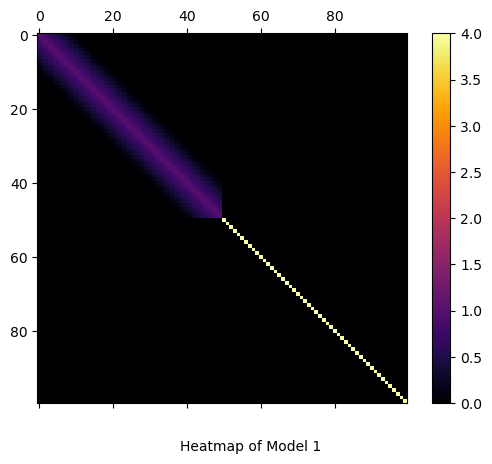
\includegraphics[scale=0.75]{simulation_result/pic_model1.png}
        \caption{Typical heatmap of Model 1 (banded matrix with ordering)}
        \label{fig:model1}
    \end{figure}
    \item Model 2 (sparse matrix without ordering). $\Sigma = \diag(A_1, A_2)$, where $A_2 = 4 I_{\frac{N}{2} \times \frac{N}{2}}$, $A_1 = B + \epsilon I_{\frac{N}{2} \times \frac{N}{2}}$, $B = [b_{ij}]_{\frac{N}{2} \times \frac{N}{2}}$, whose elements independently follow:
    \begin{equation}
        b_{ij} = \begin{cases}
            \text{Ber}(1, \frac{20}{N}) &\text{for}\hspace{2mm} i<j, \\
            1 & \text{for}\hspace{2mm}i=j, \\
            b_{ji} & \text{for}\hspace{2mm}i>j.
        \end{cases}
    \end{equation}
     Here $\text{Ber}(1, p)$ is a Bernoulli random variable that takes value 1 with probability $p$ and value 0 with probability $1-p$, and $\epsilon = \max(-\lambda_{\min} (B), 0) + 0.01$ to ensure that $A_1$ is positive definite. 
        \begin{figure}[H]
        \centering
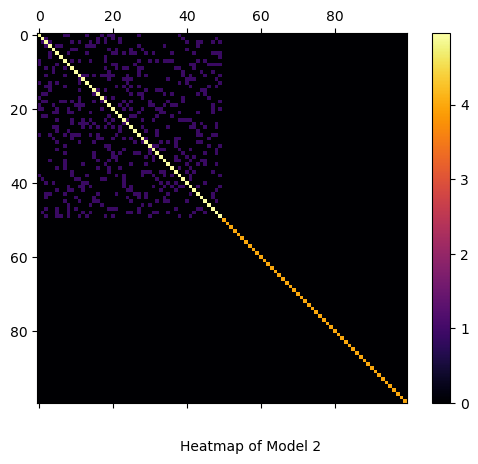
\includegraphics[scale=0.75]{simulation_result/pic_model2.png}
         \caption{Typical heatmap of Model 2 (sparse matrix without ordering)}
        \label{fig:model2}
    \end{figure}
\end{enumerate}

\subsection{Auxiliary Information}
In the simulation, we directly generate the estimates of the Location Indicator Matrix $L$ and the Relative Importance Indicator Matrix $C$, i.e., $\hat L$ and $\hat C$. The qualities of these estimates are tuned by some hyper-parameters. Table \ref{param-hatL} and \ref{param-hatC} list the descriptions of these hyper-parameters and the ranges of values they can take.
\begin{table}[htbp]
     \centering
     \begin{tabularx}{\textwidth}{c|X|c}
          \toprule
          Parameter & Description & Range \\ 
          \midrule
          \(l\) & Observation level, determines how we classify a pair \((i,j)\) as important, i.e., \(L_{ij} =1\). & 0.2 \\
          \(p\) & Conditional on \(L_{ij} =1\), the probability of actually observing \(\hat{L}_{ij} =1\). & 0.5, 0.8, 1 \\
          \(q\) & Conditional on \(L_{ij} = 0\), the probability of  observing \(\hat{L}_{ij} =1\). & 0, 0.1 \\
          \bottomrule
     \end{tabularx}
     \caption{hyper-parameters for Network Guided Thresholding Estimator}
     \label{param-hatL}
\end{table}
\vspace{10mm}
\begin{table}[htbp]
     \centering
     \begin{tabularx}{\textwidth}{c|X|c}
          \toprule
          Parameter & Description & Range \\ 
          \midrule
          $\eta$ & Accuracy rate of the order,  guarantees $S^{c_i}_{\lceil \eta k \rceil} \subseteq S^{\hat{c}_i}_{k}$ for all $1 \le k \le N$, where $c_i$ is the $i$-th column of $C$ and $\hat{c}_i$ is the $i$-th column of $\hat C$. Details of the algorithm to generate $\hat C$ can be found in \autoref{algo}.  & 0.1, 0.5, 0.8, 1 \\
          \bottomrule
     \end{tabularx}
     \caption{hyper-parameters for Network Guided Banding Estimator}
     \label{param-hatC}
\end{table}

\subsection{Numerical Results}
For each model described in \autoref{true_cov}, $T=100$ iid $N$-variate random vectors are generated from the normal distribution with mean 0 and covariance matrix $\Sigma$, for $N = 100, 300, 500$. For each setting of $(N, T, l, p, q)$ or $(N, T, \eta)$, 20 replications are used. We compare the numerical performance of the Network Guided Thresholding Estimator and the Network Guided Banding Estimator with a set of pure statistical methods including Sample Covariance Estimator, Soft Thresholding Estimator, Hard Thresholding Estimator, Linear Shrinkage Estimator, and Nonlinear Shrinkage Estimator. \autoref{res-model1} and \autoref{res-model2} list the numerical results under the Frobenius norm and the Matrix 2-norm. 

When the true covariance matrix is a banded one with order (model 1), both Network Guided estimators outperform other competitors as long as the auxiliary network information is decent. For the Network Guided Thresholding Estimator, it outperforms the sample covariance estimator, the hard thresholding estimator, and the linear shrinkage estimator for all $(p,q, N,T)$ combinations. However, to beat the soft thresholding estimator and the nonlinear shrinkage estimator, we will need $p,q$ to be not too large. In particular, type I error $q$ hurts the performance of the Network Guided Thresholding Estimator more than type II error $(1-p)$. When $q=0$, even if the probability of making the type II error is as large as $50\%$, it still performs better than other pure statistical methods. When it comes to the Network Guided Banding Estimator, it has smaller norms than all other pure statistical methods as long as the accuracy rate parameter $\eta$ is not too small. When $\eta=0.5$, the Network Guided Banding Estimator outperforms for most of the $(N,T)$ combinations. Given similar information quality, the Network Guided Banding Estimator performs better than the Network Guided Banding Estimator, which is consistent with the theory. We do not aim to compare the performances of the two Network Guided estimators as this is not a fair competition (the Network Guided Banding Estimator requires the auxiliary information to reveal the relative importance of neighbors for each node for this method to be applicable).

When the true covariance matrix is a sparse matrix without order (model 2), both Network Guided estimators again outperform other competitors when the auxiliary network information is decent. Now that our Network Guided Banding Estimator is applicable to a wider range of "bandable" matrix, it can be successfully applied under the setting of model 2. And it maintains its excellent performance given that the accuracy rate parameter $\eta$ is not too small. When $\eta=0.5$, the Network Guided Banding Estimator outperforms others for all the $(N,T)$ combinations. Even when $\eta=0.1$, its performance is still decent under this model setting. Similar to the previous setting, the Network Guided Thresholding Estimator as we are not making too much Type I error.  In summary, our simulation exercise shows the excellent numerical properties of the proposed Network Guided estimators. They both outperform other competitors as long as the auxiliary network information is decent. The performance of the Network Guided Thresholding Estimator is more sensitive to type I error than type II error. The Network Guided Banding Estimator, on the other hand, is not too sensitive to the accuracy rate parameter $\eta$, and it has excellent performance as long as $\eta$ is not too small.

\begin{landscape}
    % \resizebox{!}{0.45\textheight}{
        \begin{table}[H]
\centering
\caption{Simulation Results of Model 1}
\label{res-model1}
\resizebox{\linewidth}{0.2\textheight}{ %%%
% \resizebox{!}{0.9\textheight}{
\begin{tabular}{ll|p{2cm}p{2cm}p{2cm}p{2cm}p{2cm}p{2cm}p{2cm}p{2cm}p{2cm}p{2cm}p{2cm}p{2cm}p{2cm}p{2cm}p{2cm}}
\toprule
              &     & Network Guided Banding($\eta=1$) & Network Guided Banding ($\eta=0.8$) & Network Guided Banding ($\eta=0.5$) & Network Guided Banding ($\eta=0.1$) & Network Guided Thresholding ($(l, p, q)=(0.2, 1, 0)$) & Network Guided Thresholding ($(l, p, q)=(0.2, 1, 0.1)$) & Network Guided Thresholding ($(l, p, q)=(0.2, 0.8, 0)$) & Network Guided Thresholding ($(l, p, q)=(0.2, 0.8, 0.1)$) & Network Guided Thresholding ($(l, p, q)=(0.2, 0.5, 0)$) & Network Guided Thresholding ($(l, p, q)=(0.2, 0.5, 0.1)$) &       Sample & Soft Threshold & Hard Threshold & Linear Shrink & Nonlinear Shrink \\
Norm & $N$ &                                   &                                     &                                     &                                     &                                                       &                                                         &                                                         &                                                           &                                                         &                                                           &              &                &                &               &                  \\
\midrule
Frobenius Norm & 100 &                        5.73(0.30) &                          6.62(0.27) &                          8.84(0.39) &                         14.51(0.37) &                                            5.93(0.63) &                                              7.24(0.50) &                                              7.25(0.37) &                                                8.27(0.35) &                                              7.97(0.38) &                                                8.88(0.36) &  14.51(0.37) &     8.80(0.42) &    13.35(0.44) &   12.20(0.22) &       7.50(0.36) \\
              & 300 &                        7.96(0.22) &                         10.69(0.38) &                         15.41(0.38) &                         28.08(1.00) &                                           14.43(0.88) &                                             19.39(0.67) &                                             17.81(0.34) &                                               21.88(0.29) &                                             19.51(0.29) &                                               23.21(0.25) &  43.47(0.33) &    21.40(0.27) &    38.23(0.40) &   28.99(0.10) &             None \\
              & 500 &                        9.52(0.25) &                         13.45(0.27) &                         19.60(0.45) &                         36.45(1.04) &                                           22.26(0.65) &                                             31.18(0.53) &                                             27.56(0.47) &                                               34.96(0.41) &                                             30.10(0.43) &                                               36.87(0.39) &  72.42(0.42) &    32.82(0.41) &    62.41(0.55) &   41.31(0.10) &             None \\
Matrix-2 Norm & 100 &                        2.61(0.24) &                          2.64(0.35) &                          3.59(0.42) &                          4.48(0.52) &                                            1.77(0.25) &                                              2.02(0.24) &                                              2.09(0.27) &                                                2.31(0.25) &                                              2.39(0.39) &                                                2.54(0.37) &   4.48(0.52) &     3.18(0.45) &     3.90(0.44) &    3.75(0.37) &       3.55(0.43) \\
              & 300 &                        3.21(0.25) &                          3.82(0.34) &                          5.15(0.44) &                          7.73(0.57) &                                            2.74(0.25) &                                              3.42(0.21) &                                              3.36(0.16) &                                                3.96(0.15) &                                              3.63(0.16) &                                                4.19(0.16) &   9.24(0.34) &     3.94(0.23) &     7.37(0.21) &    5.60(0.21) &             None \\
              & 500 &                        3.21(0.28) &                          3.70(0.32) &                          5.36(0.41) &                          8.06(0.30) &                                            3.52(0.15) &                                              4.48(0.18) &                                              4.39(0.15) &                                                5.23(0.18) &                                              4.75(0.16) &                                                5.55(0.19) &  12.90(0.33) &     4.90(0.17) &    10.13(0.32) &    6.24(0.11) &             None \\
\bottomrule
\end{tabular}
}
\end{table}

        \begin{table}[H]
\centering
\caption{Simulation Results of Model 2}
\label{res-model2}
\resizebox{\linewidth}{0.2\textheight}{ %%%
\begin{tabular}{ll|p{2cm}p{2cm}p{2cm}p{2cm}p{2cm}p{2cm}p{2cm}p{2cm}p{2cm}p{2cm}p{2cm}p{2cm}p{2cm}p{2cm}p{2cm}}
\toprule
              &     & Network Guided Banding ($\eta=1$) & Network Guided Banding ($\eta=0.8$) & Network Guided Banding ($\eta=0.5$) & Network Guided Banding ($\eta=0.1$) & Networked Guided Thresholding ($(l, p, q)=(0.2, 1, 0)$) & Networked Guided Thresholding ($(l, p, q)=(0.2, 1, 0.1)$) & Networked Guided Thresholding ($(l, p, q)=(0.2, 0.8, 0)$) & Networked Guided Thresholding ($(l, p, q)=(0.2, 0.8, 0.1)$) & Networked Guided Thresholding ($(l, p, q)=(0.2, 0.5, 0)$) & Networked Guided Thresholding ($(l, p, q)=(0.2, 0.5, 0.1)$) &        Sample & Soft Threshold & Hard Threshold & Linear Shrink & Nonlinear Shrink \\
Norm & $N$ &                                   &                                     &                                     &                                     &                                                         &                                                           &                                                           &                                                             &                                                           &                                                             &               &                &                &               &                  \\
\midrule
Frobenius Norm & 100 &                        9.95(0.26) &                         10.88(0.27) &                         14.69(0.22) &                         19.57(0.40) &                                             10.35(1.65) &                                               12.83(1.29) &                                               16.22(0.60) &                                                 17.56(0.59) &                                               17.84(0.57) &                                                 18.95(0.56) &   25.94(0.49) &    19.03(0.52) &    25.71(0.51) &   16.26(0.27) &      15.20(0.32) \\
              & 300 &                       16.91(0.31) &                         18.52(0.35) &                         24.30(0.28) &                         33.88(0.27) &                                             26.82(4.30) &                                               36.72(2.80) &                                               45.48(0.92) &                                                 50.98(0.83) &                                               50.26(0.87) &                                                 54.94(0.82) &   83.47(0.63) &    53.95(0.70) &    81.89(0.68) &   33.76(0.10) &             None \\
              & 500 &                       20.39(0.30) &                         22.10(0.29) &                         30.03(0.19) &                         43.37(0.09) &                                             36.56(6.83) &                                               55.55(4.45) &                                               69.88(1.26) &                                                 79.87(1.04) &                                               76.96(0.85) &                                                 85.64(0.80) &  137.19(0.60) &    82.93(0.71) &   133.60(0.66) &   44.59(0.07) &             None \\
Matrix-2 Norm & 100 &                        3.52(0.28) &                          3.61(0.35) &                          5.13(0.35) &                          8.65(0.50) &                                              3.01(0.61) &                                                3.42(0.59) &                                                4.43(0.45) &                                                  4.73(0.46) &                                                4.81(0.43) &                                                  5.06(0.44) &    7.05(0.59) &     5.00(0.41) &     6.98(0.59) &    6.82(0.66) &       5.67(0.89) \\
              & 300 &                        3.66(0.15) &                          3.66(0.17) &                          5.09(0.22) &                          9.05(0.25) &                                              5.00(0.80) &                                                6.12(0.67) &                                                8.35(0.47) &                                                  9.17(0.47) &                                                9.18(0.51) &                                                  9.91(0.51) &   15.48(0.66) &     9.58(0.51) &    15.06(0.63) &    9.08(0.23) &             None \\
              & 500 &                        3.97(0.17) &                          4.04(0.14) &                          4.58(0.16) &                          8.78(0.07) &                                              5.26(1.04) &                                                7.00(0.93) &                                               10.52(0.27) &                                                 11.76(0.26) &                                               11.59(0.21) &                                                 12.72(0.21) &   21.43(0.38) &    12.25(0.25) &    20.58(0.36) &    9.41(0.13) &             None \\
\bottomrule
\end{tabular}
}
\end{table}

    % }
\end{landscape}

